\section{Анализ предметной области}
\subsection{Характеристика СКУД и её назначение}

История контроля доступа гораздо интереснее, чем вы думаете. На протяжении всей истории человечества мы наблюдаем за тем, как в нем используются элементы безопасности. Механические деревянные замки были обнаружены на территории современного Ирака еще в 4000 году до н. э., а гробница фараона Тутанхамона была заперта с помощью веревочного узла. Исторически контроль доступа включал в себя нечто большее, чем просто замки. У стражников королевства были сложные смены, которые позволяли им находиться в определенных местах только в определенное время, чтобы обеспечить круглосуточную охрану. Удивительно, что такие устаревшие технологии, как рвы, разводные мосты и сторожевые башни, когда-то были самыми современными инженерными решениями, используемыми для обеспечения защиты периметра и контролируемого доступа.

Сегодня под термином СКУД (Система контроля и управления доступом) понимается вид физической безопасности, который управляет точками входа в ваш бизнес или внутренние помещения здания. Простой пример СКУД -- ворота, физически не допускающие неавторизованных пользователей и позволяющие войти только авторизованным пользователям.

В наше время контроль доступа является сложным процессом, применяющимся для защиты мест, имущества, данных или граждан от личных до огромных корпоративных масштабов.  Современные достижения в области технологий позволили создать более надежные и эффективные способы управления и защиты, и современные решения по контролю доступа выходят далеко за рамки стандартных ключей и карт доступа. 

Удаленное управление остается важнейшей задачей с начала 2020 года, позволяя предприятиям обеспечивать безопасность своих зданий, даже когда там никого нет, и прокладывая путь к продуктивным гибридным моделям работы. Удаленный доступ и управление безопасностью позволяют как корпоративным, так и небольшим организациям оставаться гибкими, позволяя командам выполнять повседневные задачи без необходимости физического присутствия на объекте. Такие функции, как удаленное отпирание дверей, полезны для того, чтобы впустить в здание поставщиков, подрядчиков и сотрудников, которые забыли или потеряли свои учетные данные. Благодаря доступу к отчетам о деятельности в режиме реального времени удаленное управление также позволяет организациям гибко перестраиваться на ходу. 

Три лидера отрасли, каждый из которых разработал инновационные системы контроля доступа -- Keyscan, HID и RBH Access Technologies разрабатывают передовые системы безопасности, которые являются универсальными, масштабируемыми и гибкими, оставаясь при этом высокофункциональными.

\subsection{Ключевые элементы системы контроля доступа и принцип их работы}
\subsubsection{Учётные данные}

Учетные данные контроля доступа используют RFID (радиочастотной идентификации) для передачи сигналов на панель контроля доступа. Каждая метка имеет уникальный зашифрованный идентификационный номер. Вы можете выдать всем сотрудникам метки одного типа, но при этом настроить одну метку на разрешение входа, а другую - на запрет входа в определенные зоны здания.

УД бывают следующих видов:

\begin{itemize}
	\item Приложения для смартфонов
	\item Пароль или пин-код
	\item Биометрия
	\item Брелок или карта доступа
\end{itemize}

\paragraph{Приложения для смартфонов}

Для контроля доступа с помощью мобильных устройств используются смартфоны, планшеты и носимые электронные устройства, которые служат удостоверением личности пользователя для входа в офис или другие деловые помещения. Поскольку все больше работодателей поощряют тенденцию Bring Your Own Device (BYOD), контроль доступа с помощью приложений становится отличным инструментом для обеспечения дополнительного уровня безопасности в любой организации. В настоящее время электронные устройства даже позволяют осуществлять биометрическую аутентификацию без необходимости инвестировать в дорогостоящие биометрические считыватели.

\paragraph{Пароль или ПИН-код}

Преимущество парольных систем по сравнению с системами дискреционного контроля доступа на основе матрицы доступа заключается в том, что в них нет объекта, связанного с монитором безопасности, который хранит информацию о контроле доступа к конкретным объектам.Кроме того, парольные системы обеспечивают безопасность даже в том случае, если посторонние лица имеют неограниченный или технически возможный доступ к носителям, на которых записаны и хранятся зашифрованные объекты.Эти преимущества парольных систем управления доступом делают их чрезвычайно широко распространенными в документальных информационных системах.

\paragraph{Биометрия}

Объекты со строгими требованиями к соблюдению норм и правил, такие как больницы и производственные предприятия, требуют особенно надежных систем контроля доступа и безопасности. Биометрические технологии используют измерения тела и физические характеристики для поиска уникальных идентификационных признаков человека (обычно отпечатков пальцев, сканирования сетчатки глаза или лица), чтобы сделать идентификацию положительной. 

\paragraph{Брелок или карта доступа}

Системы контроля доступа на основе карт играют важную роль в защите вашей собственности. Системы доступа без ключа - это эффективный и доступный способ обеспечить безопасность людей, помещений и данных. Карточные системы доступа могут стать отличным выбором, независимо от того, охраняете ли вы склад, общежитие или коммерческое здание.

Простейшая современная СКУД состоит из:

\begin{itemize}
	\item Считывателя
	\item Контроллера
	\item Замка
\end{itemize}

\subsubsection {Считыватель}

Считыватель меток устанавливается на одной или обеих сторонах двери - на одной стороне двери, если система контролирует только вход, или на обеих сторонах, если система контроля доступа контролирует вход и выход. Считыватель содержит антенну, которая подключается к панели контроля доступа и получает от нее питание.
Когда человек входит в здание со своей меткой контроля доступа, на антенну считывателя поступает его зашифрованный идентификационный номер.

\subsubsection {Контроллер}

Контроллер - это ядро системы. В нем хранится информация об авторизации, которая настраивается администратором системы. Контроллер получает зашифрованный номер метки от считывателя, расшифровывает его, затем сравнивает ID-номер с ID-номерами, которые были загружены в систему. Если номера совпадают, и пользователь имеет право доступа к двери, дверь разблокируется.

\subsubsection {Замок}

Панель управления доступом, или контроллер, управляет электрическим замком двери. Если пользователю разрешено войти в здание, дверь автоматически разблокируется и может быть открыта.
Общая схема устройства системы изображена на рисунке ~\ref{fig:commonscheme1}.
\begin{figure}
	\centering
	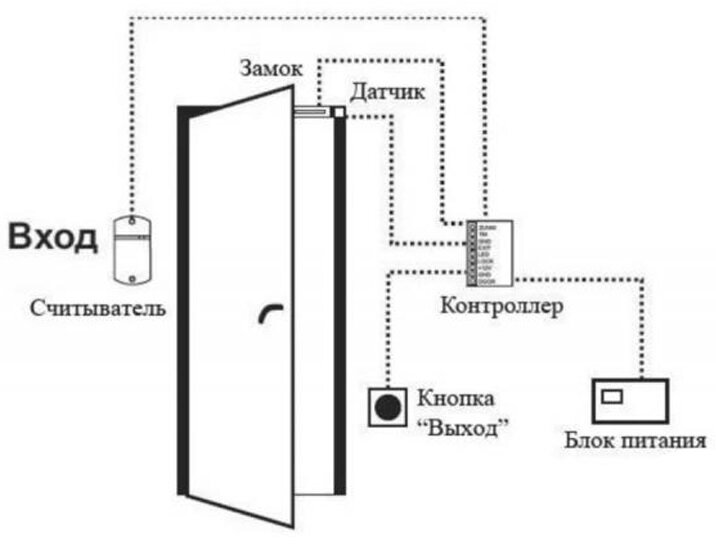
\includegraphics[width=0.7\linewidth]{images/CommonScheme1}
	\caption{Схема устройства современной СКУД}
	\label{fig:commonscheme1}
\end{figure}

\subsection{Анализ аудитории пользователей}

Система контроля и управления доступом - важный аспект безопасности. Она обеспечивает дополнительный уровень защиты, позволяя контролировать и отслеживать, кто имеет доступ к объекту защиты.

СКУД применима во многих отраслях - в здравоохранении, корпоративном, образовательном и государственном секторах. Сегодня они также применяются на различных объектах, таких как стационарные, долговременные и жилые учреждения, больницы, муниципалитеты, кондоминиумы, распределительные комплексы, малые и крупные предприятия, а также колледжи и университеты.

Среди аудитории пользователей программного обеспечения СКУД -- сисадмины и специалисты по информационной безопасности, нанятые организацией специально для контроля правил системы, устранения неполадок, проведения аудитов безопасности, поддержания работоспособности, внесения изменений.

В нашем случае, на круизном лайнере, аудиторией приложения является человек из экипажа, занимающийся внесением данных пассажиров в базу, наложением штрафов, созданием правил для входа в те или иные сектора, манипуляцией дверьми во время ЧС и т.д.

\subsection{Перспективы развития}
В перспективе развития СКУД на круизном лайнере ключевым является масштабирование её возможностей. Для самой системы это может быть увеличение быстродействия, расширение пула правил и ограничений, добавление умных систем обнаружения (камер) для фиксации нарушений и автоматического наложения штрафов, внедрение технической поддержки в реальном времени для нерядовых случаев.

В перспективе развития ПО для СКУД ключевым является наиболее точное отражение функций системы для воздействия на них со стороны специалиста.

В будущем можно рассмотреть интеграцию бэкенда в виде набора новых бизнес-правил, дополнительного уровня защиты базы данных от атак злоумышленников, таких как SQL-инъекции, а фронтенда – как более широкую реализацию библиотеки \textquotedbl tkinter \textquotedbl, что обеспечит более гибкое управление ресурсами и улучшит масштабируемость приложения.

От веревок и деревянных замков до облачных систем и биометрии - безопасность прошла долгий путь сквозь века. Аутентификация повсюду - от самых больших и надежных объектов до телефона в вашем кармане. При взгляде на будущие тенденции в области контроля доступа можно с уверенностью сказать одно: инновации, интеграция и адаптивность необходимы, но не в ущерб безопасности. Будущее контроля доступа, особенно для предприятий, выходит за рамки защиты данных и ограничения доступа и позволяет делать все это быстрее и с большей надежностью.   

\subsection{Сценарий проекта. Неформальное представление предметной области}

У нас небольшая фирма, занимающаяся разработкой СКУД. Мы выиграли контракт на разработку СКУД для небольшого круизного лайнера AIDABlu.

В основные функции СКУД входит: идентификация лиц и объектов (транспортных средств), имеющих право доступа на объект, регистрация входа-выхода (въезда-выезда), управление уровнями доступа для персонала. В СКУД входят все сущности, так или иначе связанные с предоставлением доступа. В данные сущности входят: Пассажиры, Двери, Комнаты, Штрафы. У каждой двери есть свод правил, определяющих, открыть ли её пассажиру или нет.

В обязанности CКУД входит: Контроль доступа (ДОСТУПЫ) в обычном режиме и в случае ЧС(ДОСТУПЫ-ЧС). Доступ каждого пассажира(ПАССАЖИРЫ) к каждой двери(ДВЕРИ) предоставляется/не предоставляется на основе данных ограничений пассажира и двери.  Дверь может вести в комнату(КОМНАТЫ), также имеющую данные ограничений для предоставления доступа. В процессе поездки пассажир может получить штраф(ШТРАФЫ), что является отдельным ограничением, закреплённым за пассажиром. Так как не все пассажиры могут являться совершеннолетними(ДЕТИ), за ними должен быть закреплён взрослый сопровождающий, несущий за него ответственность на время поездки.

\subsection{Бизнес-правила}

На основе анализа неформального описания предметной области были сформулированы бизнес-правила, представленные в таблице  \ref{brules:table}.

\begin{xltabular}{\textwidth}{|c|X|X|}
	\caption{Бизнес-правила\label{brules:table}}\\ \hline
	~  & \centrow  Бизнес-правило & \centrow Ограничение \\ \hline
	\endfirsthead
	\continuecaption{Продолжение таблицы \ref{brules:table}}
	~ & \centrow Бизнес-правило & \centrow Ограничение \\ \hline 
	\finishhead
	1. & Каждый человек на борту имеет постоянный доступ к жизненно-необходимым дверям:(коридорные и лестничные, туалет, собственный номер, столовая, выход на площадку, медпункт, детская комната, \textquotedbl Дьюти-фри\textquotedbl)
	& Помещение переполнено, шторм(для площадки), отсутствие несовершеннолетнего спутника(дет.комната), пол (каждому – свой туалет). В этом случае доступ не предоставляется. \\ \hline 
	2.  & Доступ к комнатам идёт далее по иерархической системе. Так, пользователи «комфорта» получают доступ к: (бару, аквапарку, кинотеатру, кальянной, бильярдной, банкетному залу, тиру) 
	& Возраст(бар/кальянная), мед. Ограничения (аквапарк), время(банкетный зал), судимости (тир),штрафы, накладываемые после проишествий. \\ \hline 
	3. & Кроме вышеперечисленного, пользователям «Все включено» открывается доступ к: (SPA, пентхаусу, рыболовной площадке, комнате для погружений, VIP-кинотеатру)
	& Мед.ограничения(пассажир может посетить SPA, если того требует здоровье и не может посещать комнату для погружений). \\ \hline 
	4. & Персонал имеет доступ ко всем дверям & Персонал не имеет доступа к личным номерам пассажиров \\ \hline
	5. & Пассажир может менять тариф в процессе путешествия & Это происходит в случае ЧС или доплаты персоналу. А в случае персонала – при отстранении от полномочий на время поездки(Тариф меняется на «эконом»). \\ \hline
	6. & Штраф пассажира может быть снят & Только если штраф относится к снимаемым, прошли 1 сутки с момента наложения и пассажир заплатил выкуп за снятие штрафа. \\ \hline
	7. & Каждый человек на борту должен иметь свой пропуск & Количество пропусков на каждого человека не должно превышать 1 \\ \hline
	8. & Несовершеннолетние также имеют свой пропуск & Для разблокировки пропуска, за ним должен быть закреплён сопровождающий \\ \hline
	9. & Ограничения пассажира могут быть как постоянными, так и наоборот & К ограничениям, которые не меняются и не оспариваются во время поездки относятся: Судимости и мед.ограничения \\ \hline
	10. & У каждого пассажира должна быть своя комната & Пассажир может войти только в ту жилую комнату, что закреплена за ним \\ \hline
	11. & В случае возникновения ЧС, СКУД начинает работать в другом режиме & В случае шторма все двери наружу закрываются (состояние), двери лестниц/коридоров всегда открыты, дабы не создавать давки и паники. \\ \hline
\end{xltabular}